\documentclass[12pt, a4paper, oneside]{ctexart}
\usepackage{amsmath, amsthm, amssymb, bm, color, graphicx, geometry, mathrsfs,extarrows, braket, booktabs, array}
\usepackage[colorlinks,linkcolor=red,anchorcolor=blue,citecolor=blue,urlcolor=blue,menucolor=black]{hyperref}
%\setCJKmainfont{SimSun}[ BoldFont = 思源宋体 Heavy, ItalicFont = KaiTi ]
%\setCJKmainfont{方正新书宋_GBK.ttf}[ BoldFont = 思源宋体 Heavy, ItalicFont = KaiTi ]
\setCJKmainfont{方正新书宋_GBK.ttf}
\setmainfont{Times New Roman}  % 设置英文字体
\setsansfont{Calibri}
\setmonofont{Consolas}

\linespread{1.4}
%\geometry{left=2.54cm,right=2.54cm,top=3.18cm,bottom=3.18cm}
\geometry{left=1.84cm,right=1.84cm,top=2.18cm,bottom=2.18cm}
\newcounter{problem}  % 问题序号计数器
\newenvironment{problem}{\stepcounter{problem}\par\noindent\textbf{题目\arabic{problem}. }}{\smallskip\par}
\newenvironment{solution}{\par\noindent\textbf{解答. }}{\smallskip\par}
\newenvironment{note}{\par\noindent\textbf{注记. }}{\smallskip\par}

%%%% 图片相对路径 %%%%
\graphicspath{{figure/}} % 当前目录下的figure文件夹, {../figure/}则是父目录的figure文件夹

\everymath{\displaystyle} % 默认全部行间公式
\DeclareMathOperator*\uplim{\overline{lim}} % 定义上极限 \uplim_{}
\DeclareMathOperator*\lowlim{\underline{lim}} % 定义下极限 \lowlim_{}
\let\leq=\leqslant % 将全部leq变为leqslant
\let\geq=\geqslant % geq同理

%%%% 一些宏定义 %%%%
\def\bd{\boldsymbol}        % 加粗(向量) boldsymbol
\def\disp{\displaystyle}    % 使用行间公式 displaystyle(默认)
\def\tsty{\textstyle}       % 使用行内公式 textstyle
\def\sign{\text{sign}}      % sign function
\def\wtd{\widetilde}        % 宽波浪线 widetilde
\def\R{\mathbb{R}}          % Real number
\def\N{\mathbb{N}}          % Natural number
\def\Z{\mathbb{Z}}          % Integer number
\def\Q{\mathbb{Q}}          % Rational number
\def\C{\mathbb{C}}          % Complex number
\def\d{\mathrm{d}}          % differential operator
\def\e{\mathrm{e}}          % Euler's number
\def\i{\mathrm{i}}          % imaginary number
\def\re{\mathrm{Re}}        % Real part
\def\im{\mathrm{Im}}        % Imaginary part
\def\res{\mathrm{Res}}      % Residue
\def\L{\mathcal{L}}         % Loss function
\def\wdh{\widehat}          % 宽帽子 widehat
\def\ol{\overline}          % 上横线 overline
\def\ul{\underline}         % 下横线 underline
\def\add{\vspace{1ex}}      % 增加行间距
\def\del{\vspace{-3.5ex}}   % 减少行间距

%%%% 定理类环境的定义 %%%%
\newtheorem{theorem}{定理}

%%%% 基本信息 %%%%
\newcommand{\RQ}{\today} % 日期
\newcommand{\km}{泛函分析} % 科目
\newcommand{\bj}{强基数学002} % 班级
\newcommand{\xm}{吴天阳} % 姓名
\newcommand{\xh}{2204210460} % 学号

\begin{document}

%\pagestyle{empty}
\pagestyle{plain}
\vspace*{-15ex}
\centerline{\begin{tabular}{*5{c}}
    \parbox[t]{0.25\linewidth}{\begin{center}\textbf{日期}\\ \large \textcolor{blue}{\RQ}\end{center}} 
    & \parbox[t]{0.2\linewidth}{\begin{center}\textbf{科目}\\ \large \textcolor{blue}{\km}\end{center}}
    & \parbox[t]{0.2\linewidth}{\begin{center}\textbf{班级}\\ \large \textcolor{blue}{\bj}\end{center}}
    & \parbox[t]{0.1\linewidth}{\begin{center}\textbf{姓名}\\ \large \textcolor{blue}{\xm}\end{center}}
    & \parbox[t]{0.15\linewidth}{\begin{center}\textbf{学号}\\ \large \textcolor{blue}{\xh}\end{center}} \\ \hline
\end{tabular}}
\vspace*{4ex}

% 正文部分
\begin{problem}
    证明$(C(M),\rho)$为完备的度量空间.($\rho(f, g) = \max_{x\in M}|f(x) - g(x)|$,列紧集$M$上的度量记为$d$)
\end{problem}
\begin{proof}
    首先证明$(C(M),\rho)$为度量空间,由于$\rho$满足度量的基本性质,只需证明$\rho$的定义有意义,也就是证明$\forall f\in C(M)$,$f(M)$能取到最大值和最小值,下证$f(M)$为紧集.
    
    $\forall f\in C(M)$,取点列$\{y_n\}\subset f(M)$,则$\exists x_i\in M$使得$f(x_i)=y_i$,则$\{x_n\}\subset M$,由于$M$为紧集,则存在收敛子列$x_{n_k}\to x_0\in M$,由$f$的连续性可知,$f(x_{n_k})\to f(x_0)\in f(M)$. 令$y_0 = f(x_0)$,则$y_{n_k}\to y_0$,则$f(M)$为$\R$中的紧集,蕴含$f(M)$为有界闭集的数集,则$f(M)$能取到最大值和最小值,故$(C(M),\rho)$为度量空间.

    其次证明完备性,设$\{\varphi_n\}$为$C(M)$中的Cauchy列,则$\rho(\varphi_n, \varphi_m) = \max_{x\in M}|\varphi_n(x)-\varphi_m(x)|\to 0,\ (n,m\to \infty)$,任取$x_0\in M$,令$y_n = \varphi_n(x_0)$,则$|y_n-y_m|\leq \max_{x\in M}|\varphi_n(x)-\varphi_m(x)|\to 0,\ (n,m\to \infty)$,所以$\{y_n\}$为$\R$中的Cauchy列,由于$\R$是完备的,则$y_n\to y_0\in \R$,令$\varphi(x_0) = y_0= \lim_{n\to \infty}\varphi_n(x_0)$,由于$x_0$的任意性,$\varphi(x) = \lim_{n\to\infty}\varphi_n(x)$.

    下证$\varphi(x)\in C(M)$,$\forall \varepsilon > 0$,$\exists N > 0$使得$\forall n\geq N$有$|\varphi(x) - \varphi_n(x)| < \frac{\varepsilon}{3}$,由$\varphi_n$的连续性,$\forall x_0\in M$,$\exists \delta > 0$使得$\forall d(x, x_0) < \delta$,有$|\varphi_n(x) -\varphi_n(x_0)| < \frac{\varepsilon}{3}$,则
    \begin{equation*}
        |\varphi(x) - \varphi(x_0)|\leq |\varphi(x)-\varphi_n(x)|+|\varphi_n(x)-\varphi_n(x_0)|+|\varphi_n(x_0)-\varphi(x_0)| < \varepsilon
    \end{equation*}
    所以$\varphi(x)\in C(M)$,故$(C(M), \rho)$为完备的度量空间.
\end{proof}
\begin{problem}
    在度量空间$l^p(1\leq p < \infty)$中,$A\subset l^p$是列紧集,当且仅当,$A$有界,且$\forall \varepsilon > 0$,$\exists N > 0$使得$\xi = \{x_n\}\subset A$.
\end{problem}
\begin{proof}
    充分性,$A$为列紧集,则$A$为完全有界集,故$A$有界,且存在$\varepsilon$-网$\{\xi_1,\cdots, \xi_{N_{\varepsilon}}\}$使得$A\subset \bigcup_{i=1}^{N_{\varepsilon}}B(\xi_i,\varepsilon)$,则$\forall \varepsilon > 0$,$\exists N_i > 0$,使得
    \begin{equation*}
        \sum_{j\geq N_i}|x_j^{(i)}|^p < \varepsilon,\quad(1\leq i\leq N_\varepsilon, \xi_i=\{x_n^{(i)}\})
    \end{equation*}
    取$N = \max_{1\leq i\leq N_\varepsilon}N_i$,则$\sum_{j\geq N}|x_j^{(i)}|^p < \varepsilon,\ (\xi_i = \{x_n^{(i)}\})$. $\forall \xi\in l^p$,令$\xi = \{x_n\}$,则$\exists 1\leq i_0\leq N_\varepsilon$使得$\xi\in B(\xi_{i_0},\varepsilon)$则
    \begin{equation*}
        \sum_{i=N}^\infty |x_i|^p\leq \sum_{i=N}^\infty |x_i-x_i^{(i_0)}|^p + \sum_{i=N}^\infty |x_i^{(i_0)}|^p < \varepsilon^p + \varepsilon
    \end{equation*}
    
    必要性,先证明$l^p$是完备的,令$\{\xi_n\}$为$l^p$中的Cauchy列,即$\xi_i = \{x_n^{(i)}$,则$\rho(\xi_n,\xi_m) = \left(\sum_{i=1}^\infty|x_i^{(n)}+x_i^{(m)}|^p\right)^{\frac{1}{p}} \to 0$,则$|x_i^{(n)}-x_i^{(m)}|\to 0,\ (i\geq 1,\ n,m\to \infty)$. 由于$\R$是完备的,则$\exists x_i\in \R$使得$\lim_{m\to\infty}x_i^{(m)} = x_i$.
    
    令$\xi = \{x_1,x_2,\cdots\}$,由于$\{x_n^{(m)}\}\subset l^p$,则$\forall \varepsilon > 0$,$\exists N_m > 0$,使得$\sum_{i\geq N_m}|x_i^{(m)}|^p < \varepsilon$,于是有
    \begin{equation*}
        \sum_{i\geq N_m}|x_i|^p\leq \sum_{i\geq N_m}|x_i-x_i^{(m)}|^p+\sum_{i\geq N_m}|x_i^{(m)}|^p \to 0,\quad(m\to\infty)
    \end{equation*}
    所以$\xi\in l^p$. $\forall \varepsilon > 0$,$\exists N > 0$使得$\forall n \geq N$,有$|x_i^{(n)}-x_i| < \frac{\varepsilon^p}{2^{\frac{1}{p}}}$,则
    \begin{equation*}
        \rho(\xi,\xi_n)=\left(\sum_{i=1}^\infty|x_i-x_i^{(n)}|^p\right)^{\frac{1}{p}}\leq \left(\sum_{i=1}^\infty\frac{\varepsilon^p}{2^i}\right)^{\frac{1}{p}} = \varepsilon.
    \end{equation*}
    所以$\lim_{n\to\infty}\xi_n=\xi$,故$l^p$是完备的.

    下面证明$A$是完全有界集,$\forall \varepsilon > 0$,$\exists N > 0$使得$\sum_{i\geq N}|x_i|^p < \varepsilon,\ (\forall \{x_n\}\subset A)$,记$S=\{(x_1,x_2,\cdots, x_N):\{x_n\}\subset A\}\subset \R^n$,由于$A$有界,则$S$有界,由于$\R^N$中有界点列必有收敛子列,则$S$为列紧集,蕴含$S$为完全有界集,存在$\varepsilon$-网,$\{(x_1^{(1)}, \cdots, x_N^{(1)}),\cdots, (x_1^{(N_\varepsilon)},\cdots,x_N^{(N_\varepsilon)})\}$,令$\{x_n^{(i)}\}$为$\xi_i$在前$N$项的截断. 下证$\{\xi_1,\cdots, \xi_{N_\varepsilon}\}$构成$A$的$\varepsilon'$-网.

    $\forall \xi\in A$,令$\xi=\{x_n\}$,由于$(x_1,\cdots, x_N)\in S$,则$\exists i_0\in[1,N_\varepsilon]$,使得$\left(\sum_{i=1}^N|x_i-x_i^{(i_0)}|^p\right)^{\frac{1}{p}}< \varepsilon$,
    令$\varepsilon' = (\varphi^p+2\varepsilon)^{\frac{1}{p}}$,所以有
    \begin{equation*}
        \rho(\xi, \xi_{i_0}) = \left(\sum_{i=1}^\infty|x_i-x_i^{(i_0)}|^p\right)^{\frac{1}{p}}\leq \left(\sum_{i=1}^N|x_i-x_i^{(i_0)}|^p+\sum_{i=N}^\infty |x_i|^p+\sum_{i=N}^\infty|x_i^{(i_0)}|^p\right)^{\frac{1}{p}} < (\varepsilon^p+2\varepsilon)^{\frac{1}{p}} = \varepsilon'.
    \end{equation*}
    故$A$为列紧集.
\end{proof}
\begin{problem}
    令$W_0^{1,2}(0,1)$是$C_0^1(0,1)$在$\rho(f,g)=\left(\int_0^1(|f-g|^2+|f'-g'|^2)\,\d x\right)^{\frac{1}{2}}$下的完备化空间. 证明:$S = \{u\in C_0^1(0,1), \rho(u,0) < M < \infty\}$是$C[0,1]$中的列紧集.
\end{problem}
\begin{problem}
    \textbf{(1.2.3)}设$F$是只有有限项不为$0$的实数列全体,在$F$上引进距离$\rho(\xi,\eta) =\sum_{n\geq 1}|x_n-y_n|$,其中$\xi = \{x_n\}\in F, \eta = \{y_n\}\in F$,求证:$(F,\rho)$不完备,并指出它的完备化空间.
\end{problem}
\begin{proof}
    令$\xi_1 = (1,0,0,\cdots), \xi_2 = (1, \frac{1}{2}, 0,\cdots),\cdots, \xi_n=(1,\frac{1}{2},\cdots,\frac{1}{n}, 0,\cdots)$,于是$\{x_n\}\subset F$,且$\forall n, m > 0$,不妨令$m > n$,有$\rho(\xi_n, \xi_m) = \frac{1}{n+1}\to 0,\quad(n, m\to\infty)$,所以$\{\xi_n\}$为Cauchy列,但是$\lim_{n\to\infty}\xi_n\notin F$,所以$\{\xi_n\}$不收敛,则$F$不完备.

    下证$F$的完备化空间为$G = \{\{x_n\}:\lim_{n\to\infty}|x_n|=0\}$.

    $\forall \varepsilon > 0$,$\exists N >0$使得$\forall n\geq N$有$|x_n| < \varepsilon$,令$\xi = \{x_1,x_2,\cdots, x_N,0,\cdots\}\in F$,则$\rho(\xi, \eta) = \sup_{n\geq N}|x_n| < \varepsilon$,所以$F$在$G$中稠密.

    任取Cauchy列$\{\eta_n\}\subset G$,令$\eta_i = \{y_n^{(i)}\}$,则$\rho(\eta_n,\eta_m) = 0,\ (n,m\to\infty)$. $\forall \varepsilon > 0$,$\exists N > 0$使得$\forall n, m > N$有$\rho(\eta_n,\eta_m) < \varepsilon$,则$\forall i \geq 1$有$|x_i^{(n)}-x_i^{(m)}| < \varepsilon$,有$\R$的完备性可知$\exists x_i\in \R$使得$\lim_{n\to\infty}x_i^{(n)} = x_i$,令$\eta  = \{x_1,x_2,\cdots\}$,存在充分大的$m$使得$|x_i^{(m)} - x_i| < \varepsilon$,由于$\eta_m\in G$,则$\exists N_m > 0$使得$\forall i\geq N_m$有$|x_i^{(m)}| < \varepsilon$. 于是$\forall i \geq N_m$有$|x_i|\leq |x_i-x_i^{(m)}|+|x_i^{(m)}| < 2\varepsilon$,则$\eta\in G$,且$\lim_{n\to\infty}\eta_n = \eta$,故$G$为完备空间.

    故$F$在恒等变换下同构于完备空间$G$中的稠密子集,所以$G$为$F$的完备化空间.
\end{proof}
\begin{problem}
    \textbf{(1.2.5)}在完备的度量空间$(X, \rho)$中给定点列$\{x_n\}$,若$\forall \varepsilon > 0$,存在Cauchy列$\{y_n\}$,使得$\rho(x_n,y_n) < \varepsilon,\ (n\in\N)$,求证:$\{x_n\}$收敛.
\end{problem}
\begin{proof}
    $\forall \varepsilon > 0$,$\exists N >0$使得$\forall n, m \geq N$有$\rho(y_n, y_m)\leq \varepsilon$,由题意可知
    \begin{equation*}
        \rho(x_n,x_m)\leq \rho(x_n,y_n) + \rho(y_n,y_m)+\rho(y_m,x_m) < 3\varepsilon,
    \end{equation*}
    则$\{x_n\}$为Cauchy列,由$X$的完备性可知$\{x_n\}$收敛.
\end{proof}
\begin{problem}
    \textbf{(1.3.1)}在完备的度量空间$(X,\rho)$中求证:子集$A$列紧的充要条件是对$\forall \varepsilon > 0$,存在$A$的列紧的$\varepsilon$-网.
\end{problem}
\begin{proof}
    充分性,$\forall \varepsilon > 0$,存在有限$\varepsilon$-网$\{x_1,\cdots, x_N\}$,在$\R$中有界闭集即为列紧集,则$\{x_1,\cdots, x_N\}$为列紧的$\varepsilon$-网.

    必要性,$\forall \varepsilon > 0$,令$V$为$A$的列紧的$\frac{\varepsilon}{2}$-网,则$A\subset \bigcup_{y\in V}B(y,\frac{\varepsilon}{2})$,由于$V$是列紧的,则$V$是完全有界集,则存在有限的$\frac{\varepsilon}{2}$-网$\{y_1,\cdots, y_N\}$使得$V\subset \bigcup_{i=1}^NB(y_i,\frac{\varepsilon}{2})$,则$\forall a \in A$,$\exists y\in V$使得$\rho(a,y) < \frac{\varepsilon}{2}$,$\exists 1\leq i_0\leq N$使得$\rho(y,y_{i_0}) < \frac{\varepsilon}{2}$,则$\rho(a, y_{i_0})\leq \rho(a, y)+\rho(y, y_{i_0})<\varepsilon$,由$a$的任意性可知$A\subset \bigcup_{i=1}^NB(y_i,\varepsilon)$,则$\{y_1,\cdots, y_N\}$为$A$的有限$\varepsilon$-网,于是$A$为完全有界集,又由于$X$是完备的,故$A$为列紧集.
\end{proof}
\begin{problem}
    \textbf{(1.3.2)}在度量空间$(X,\rho)$中求证:紧集上的连续函数必是有界的,并且达到它的上、下确界.
\end{problem}
\begin{proof}
    (与题目1证明完全相同)设$M\subset X$为紧集,$\forall f\in C(M)$,取点列$\{y_n\}\subset f(M)$,则$\exists x_i\in M$使得$f(x_i)=y_i$,则$\{x_n\}\subset M$,由于$M$为紧集,则存在收敛子列$x_{n_k}\to x_0\in M$,由$f$的连续性可知,$f(x_{n_k})\to f(x_0)\in f(M)$. 令$y_0 = f(x_0)$,则$y_{n_k}\to y_0$,所以$f(M)$为$\R$中的紧集,蕴含$f(M)$为有界闭集的数集,则$f(M)$能达到它的上、下确界.
\end{proof}
\begin{problem}
    \textbf{(1.3.4)}设$(X,\rho)$为度量空间,$F_1,F_2$为它的两个紧子集,求证:$\exists x_i\in F_i(i=1,2)$,使得$\rho(F_1,F_2) = \rho(x_1,x_2)$,其中
    \begin{equation*}
        \rho(F_1,F_2):=\inf\{\rho(x, y):x\in F_1,y\in F_2\}.
    \end{equation*}\del
\end{problem}
\begin{proof}
    令$\rho(F_1,F_2) =A$,则存在$\{(x_n,y_n)\}$使得$\rho(x_n,y_n)\to A$,由于$F_1,F_2$为紧集,则$F_1,F_2$为自列紧集,则存在子列$x_{n_k}\to x_0\in F_1,y_{n_k}\to y_0\in F_2$,则
    \begin{equation*}
        A\leq \rho(x_0, y_0)\leq \rho(x_0, x_{n_k})+\rho(x_{n_k},y_{n_k}) + \rho(y_{n_k},y_0)\to A,\quad (k\to \infty)
    \end{equation*}
    则$\rho(x_0, y_0) = A$.
\end{proof}
\begin{problem}
    \textbf{(1.3.6)}$E = \{\sin nt\}_{n=1}^\infty$,求证:$E$在$C[0,\pi]$中不是列紧的.
\end{problem}
\begin{proof}
    只需证明$E$在$C[0,\pi]$中不是等度连续的. 令$\varepsilon = \frac{1}{2}$,$\delta = \frac{2}{n}$,取$t_1 = 0, t_2 =\frac{\pi}{2n}$,则$\forall n > 0$,有$|t_1-t_2| = \frac{\pi}{2n}<\frac{2}{n}=\delta$,且$|\sin nt_2-\sin nt_1| = 1 > \varepsilon$,所以$E$在$C[0,1]$中不是等度连续,\add 则$E$在$C[0,\pi]$中不是列紧集.
\end{proof}
\begin{problem}
    \textbf{(1.3.7)}$S = \{\xi = \{x_n\}:x_i\in \C, i\geq 1\}$,则$S$在度量
    \begin{equation*}
        \rho(\xi, \eta) = \sum_{k=1}^\infty \frac{1}{2^k}\frac{|x_k-y_k|}{1+|x_k-y_k|},\quad(\xi = \{x_n\},\eta = \{y_n\})
    \end{equation*}
    下是完备的. 设$A\subset S$,则$A$是列紧的充要条件为:$\forall n\in \N, \exists C_n > 0$,使得对于$\forall \xi = \{x_n\}\in A$有$|x_n|\leq C_n$.
\end{problem}
\begin{proof}
    充分性,反设,$\exists n_0\in \N$使得$\forall m > 0$,$\exists \xi_m = \{x_n^{(m)}\}\in A$有$|x_{n_0}^{(m)}| = m$,则在点集$E = \{\xi_n\}$中,$\forall n, m \in\N,\ n\neq m$,有
    \begin{equation*}
        \rho(\xi_n,\xi_m) \geq \frac{1}{2^{n_0}}\,\frac{1}{\frac{1}{|m-n|}+1}\geq \frac{1}{2^{n_0}}\,\frac{1}{2} = \frac{1}{2^{n_0+1}},
    \end{equation*}
    则点集$E$中无收敛子列,与$A$是列紧集矛盾,故原命题成立.

    必要性,由于$(S, \rho)$是完备的,只需证明$A$是完全有界集. $\forall N > 0$,令$E = \{(x_1,\cdots, x_N):\xi=\{x_n\}\in A\}\in \R^N$,由于$\forall n\in \N$,$\exists C_n > 0$使得$\forall \xi = \{x_n\}\in A$有$|x_n|\leq C_n$,则
    \begin{equation*}
        E\subset [-C_1,C_1]\times [-C_2,C_2]\times \cdots \times [-C_N,C_N],
    \end{equation*}
    于是$E$为$\R^N$中的有界闭集,则$E$为紧集,$\forall \varepsilon > 0$,存在$\varepsilon$-网$\{(x_1^{(1)}, \cdots, x_N^{(1)}),\cdots, (x_1^{(N_\varepsilon)}, \cdots, x_N^{(N_\varepsilon)})\}$,则$\exists \xi^{(i)}\in A$使得$(x_1^{(i)},\cdots,x_N^{(i)})$为$\xi^{(i)}$的前$N$项截断.

    $\forall \xi \in S$,令$\xi = \{x_n\}$,则$(x_1,\cdots, x_N)\in E$,则$\exists 1\leq i_0\leq N_\varepsilon$,使得$\left(\sum_{i=1}^N(x_i-x_i^{(i_0)})\right)^{\frac{1}{2}} < \varepsilon$,则
    \begin{align*}
        \rho(\xi, \xi_{i_0}) =&\ \sum_{k=1}^{\infty}\frac{1}{2^k}\,\frac{1}{\frac{1}{|x_k-x_k^{(i_0)}|}+1}\\
        =&\ \sum_{k=1}^N\frac{1}{2^k}\,\frac{1}{\frac{1}{|x_k-x_k^{(i_0)}|}+1}+\sum_{k=N+1}^\infty\frac{1}{2^k}\,\frac{1}{\frac{1}{|x_k-x_k^{(i_0)}|}+1}\\
        \leq&\ \sum_{k=1}^N\frac{\varepsilon}{2^k}+\sum_{k=N+1}^\infty \frac{1}{2^k} = \frac{2^N-1}{2^N}\varepsilon+\frac{1}{2^{N}}\to\varepsilon\quad(N\to\infty)
    \end{align*}
    则$E$为$A$的$\varepsilon$-网,则$A$为完全有界集,故$A$为列紧集.
\end{proof}
\begin{problem}
    \textbf{(1.3.9)}$(M,\rho)$为紧度量空间,$E\subset C(M)$,$E$中函数一致有界,且满足下列Hölder条件
    \begin{equation*}
        |x(t_1)-x(t_2)|\leq C\rho(t_1,t_2)^\alpha,\quad(\forall x\in E,\forall t_1,t_2\in M)
    \end{equation*}
    其中$0 < \alpha \leq 1,\ C>0$. 求证:$E$在$C(M)$中是列紧集.
\end{problem}
\begin{proof}
    只需证$E$等度连续的,$\forall \varepsilon > 0$,取$\delta < \left(\frac{\varepsilon}{C}\right)^{\frac{1}{\alpha}}$,使得$\forall \rho(t_1,t_2) < \delta$,有
    \begin{equation*}
        |x(t_1)-x(t_2)|\leq C\delta^\alpha < \varepsilon,
    \end{equation*}
    所以$E$是等度连续的,所以$E$在$C(M)$中是列紧集.
\end{proof}

% 下面给一些功能的写法
\iffalse
% 图片模板
\centerline{
    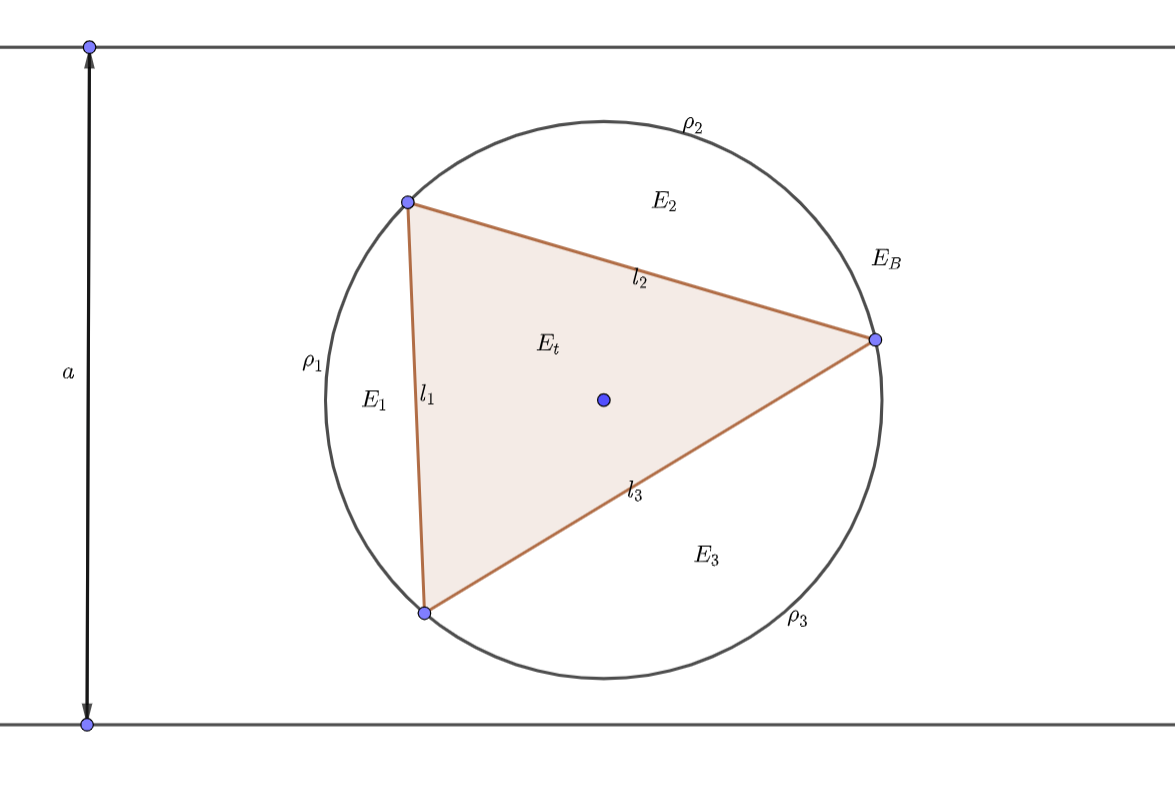
\includegraphics[width=0.8\textwidth]{figure.png}
}
% 表格模板
\renewcommand\arraystretch{0.8} % 设置表格高度为原来的0.8倍
\begin{table}[!htbp] % table标准
    \centering % 表格居中
    \begin{tabular}{p{1cm}<{\centering}p{1cm}<{\centering}p{3cm}<{\centering}p{5cm}<{\centering}} % 设置表格宽度
    %\begin{tabular}{cccc}
        \toprule
        $x_i$ & $f[x_1]$ & $f[x_i,x_{i+1}]$ & $f[x_i,x_{i+1},x_{i+2}]$ \\
        \midrule
        $x_0$ & $f(x_0)$ &                  &                          \\
        $x_0$ & $f(x_0)$ & $f'(x_0)$        &                          \\
        $x_0$ & $f(x_1)$ & $\frac{f(x_1)-f(x_0)}{x_1-x_0}$ & $\frac{f(x_1)-f(x_0)}{(x_1-x_0)^2}-\frac{f'(x_0)}{x_1-x_0}$\\
        \bottomrule
    \end{tabular}
\end{table}

\def\Log{\text{Log}} % 一个简单的宏定义
$\Log$ % 调用方法
\fi

\end{document}